% Methods
In this chapter, a description of event selection is given, as well as definitions of
key physical variables and how they are used to select events. Then, a procedure regarding
how the signal sample is manipulated to produce a high statistics off-shell tail is described.
Finally, the binning of variables used to obtain the results is determined and defined.

\section{Event selection and physical variables}
% \begin{itemize}
%     \item Description of homebrew event variables and their physical significance
%     \item DJJ\_VBF prescription
% \end{itemize}
Proton bunches cross each at a rate of about \SI{400}{\mega\hertz} in the beam line of
the LHC, naturally, not all of these crossings are recorded due to both technical
limitation of the electronics as well as the fact that the vast majority of these
crossings don't produce inelastic collision that is energetic enough to be interesting to us.

After the selection of Level 1 (L1) trigger and the higher level trigger (HLT), less than 1000
events per second are permanently recorded and would go to off-line, full reconstruction. Among these,
we only select the ones that passes certain triggers.
\todo[inline]{give a correct account for what trigger is used for 2018
TriggerHelpers::kDoubleMu, TriggerHelpers::kDoubleEle, Trigger Help.cc
TriggerHelpers::kSingleMu, TriggerHelpers::kSingleEle range pt
}

The jets are all AK4 jets unless mentioned otherwise. We shall also define a few of the
uncommon variables in the list, and a physical motivations are given in the next few
paragraphs.

After selecting mandating passing certain triggers, we make a base line cut in the variables
based on more delicate physics reason, the list of base line cuts is as below:
\begin{itemize}
    \item No ak4-jet b-tagged jet
    \item Both leptons have $p_\mathrm{T} > \SI{25}{\giga\electronvolt}$
    \item $\abs{\Delta\phi_{\ell\ell\_\met}} > 1.0$
    \item $\abs{\Delta\phi_{\ell\ell\mathrm{Jets}\_\met}} > 2.5$
    \item $\abs{m_{\ell\ell} - 91.2\gev} < 15\gev$:
        the signal process consists of $\mathrm{Z}\rightarrow{}\ell\ell$, we
        require the di-lepton system has a mass that is consistent within the Z mass peak.
    \item $p_\mathrm{T}^{\ell\ell} > 55\gev$: 
        the Drell–Yan (DY) process creates a lot of backgrounds events, but their di-leptons
        go back-to-back with expected value of this variable close to 0.
    \item $\met > 125\gev$:
        the signal process creates true $\met$ with neutrinos, this cut also reduce bkg such
        as DY.
    \item $\min{\abs{ \Delta\phi_{\mathrm{j}\_\met}}} > 0.25$
    %eta muon < 2.4
    %eta electron < 2.5
    % \item $p_\mathrm{T}^{\ell\ell} > 55\gev$
\end{itemize}
% \todo[inline]{define the uncommon ones and give account for the choice}
% \missingfigure{Show how much backgrounds are gone for maybe 2 samples}

A lot of the cuts are related to angles between various physical objects presented in the
reconstruction. The reason is simple: the signal events, where Higgs goes to ZZ and one Z
goes to 2 charged lepton the other goes to 2 neutrinos, ideally would have the two Z's 
`back-to-back' in Higgs' rest frame leading to a large angel in the transverse plane. (
assuming the $\met$ mainly comes from the two neutrinos, of course)

Furthermore, in background events which do not mandate this kinematic feature, the
correlation in the directions of $\met$ and of observable physical objects is weaker.

To use this kinematic feature to increase signal to background ratio, we define 
$\abs{\Delta\phi_{\ell\ell\_\met}}$ as the azimuthal angel (perpendicular to 
the beam line) between the di-lepton system and the transverse missing energy. In the
signal events that produce 0 jet, this variable should be $\pi$. The cut is lowered to $1.0$ 
due to the finding that in the (not so rare) case where there are jet(s) recoiling against
the ZZ system, the variable dips quite low.

This leads to the next variable on the list $\abs{\Delta\phi_{\ell\ell\mathrm{Jets}\_\met}}$, which
is almost the same except that we add all jets' momentum into the di-lepton system to account
for the events that have produced jets, which in turn would cause the angel be lower in such
a multi-body final states.

Finally, $\min{\abs{ \Delta\phi_{\mathrm{j}\_\met}}}$ is the minimum azimuthal angel difference between
any of the jet (that passes cuts) and the $\met$, it exist because jets are as mentioned, one of the 
most difficult physical objects measure, they often create so-called instrumental $\met$ due to jet
mismeasurements and it can be quite large in magnitude. However, such mismeasurements often yields large
$\met$ in the direction of the original jet. This cuts requires angular separation since in signal process,
the jet recoils against ZZ system.
\newpage\phantom{blabla}

\section{Signal samples re-weighting}
\label{sec:sig_rewgt}
% \begin{itemize}
%     \item Physics of Higgs signal sample (the weight, ME)
%     \item the need for pieceing together samples with different LHE Mass
%     \item results (also see appendix A)
% \end{itemize}
Extra attnsion was paied to the off-shell Higgs sample used in this thesis and two different kinds
of re-weigthing of the simulated events are applied in achiveing a high quality sample with wide
mass spectrum way beyong the mass of Higgs ($\approx \SI{125}{\giga\electronvolt}$). We use the
gluon fusion Higgs (ggH) sample to illustrae the procedures, the same procedures are applied to
the VBF samples as well.

We start by generating separate samples with different Higgs mass, which we call LHECandMass in the
following plots. This is the mass of Higgs terms appears in the propagator on 
the R.H.S of Eq.~\ref{eqn:diff_xsec} as mentioned before. The raw distribution of the the true mass
in different samples (without any weight) is shown in Fig.~\ref{fig:LHE_raw} (left). As expected, 
the peak of the distribution moves to the right as the mass of the sample becomes larger, at the
same time, the `peak' of samples with very large mass becomes wider becuse the the lower edge
of the peak is dominated by an underlying exponential `tail'. We also see that for some lower mass
samples (200, 300, 400 etc.), they have a cut-off beyond $\mathrm{M}\approx2500$ which means they have 0
statistics beyong that mass range. After applying the GEN, PU, and ME weights given by their
individual MC process and JHUGen MELA, as shown in Fig.~\ref{fig:LHE_raw},
we see that they are consistent with each others' line shape. However, it is clear
that:
\begin{enumerate}[label=(\roman*)]
  \item Lower mass samples have cut-offs in the tail region
  \item Samples have poor statistics in mass windows that are 
      far from their true mass (as listed in the legend).
\end{enumerate}
The second point is best illustrated by the wide spikes of lower mass samples near their cut-offs,
as well as the visible fluctuations of high-mass samples in the mass region (don't be fooled by the 
visual, the plot is in semi-log scale).
\begin{figure}[htb]
\begin{center}
\subfloat[]{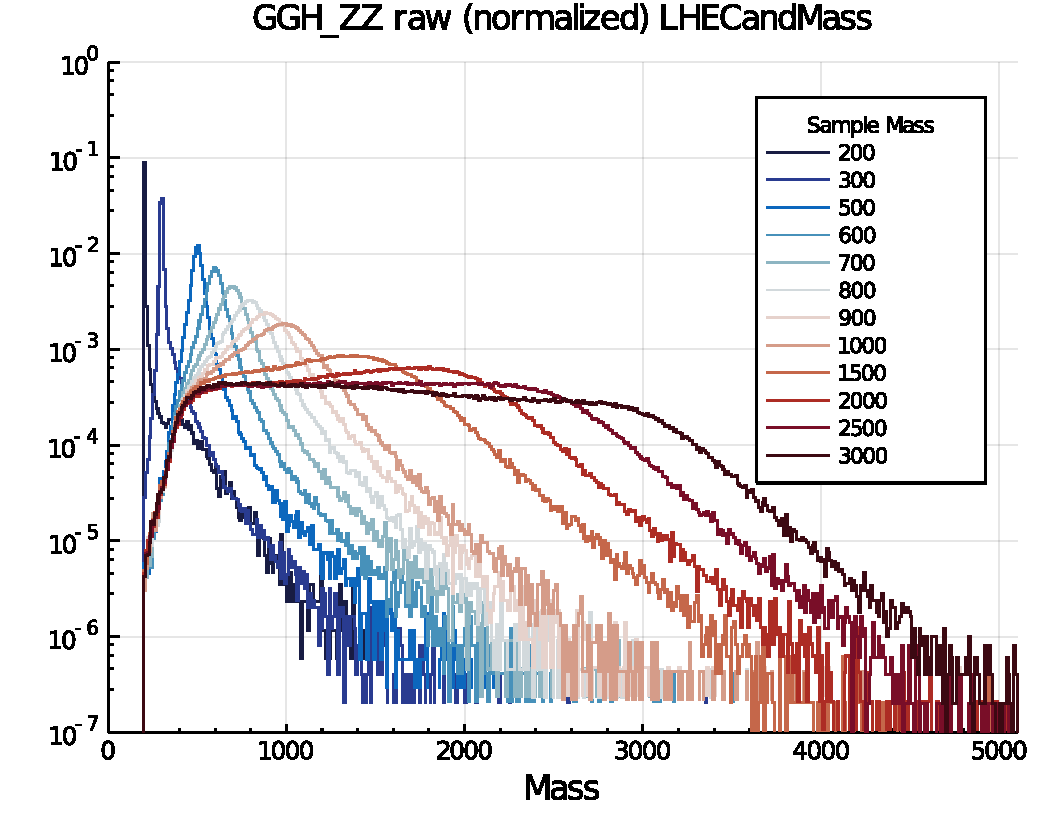
\includegraphics[width=.5\linewidth]{fig/LHE_Raw.pdf}}
\subfloat[]{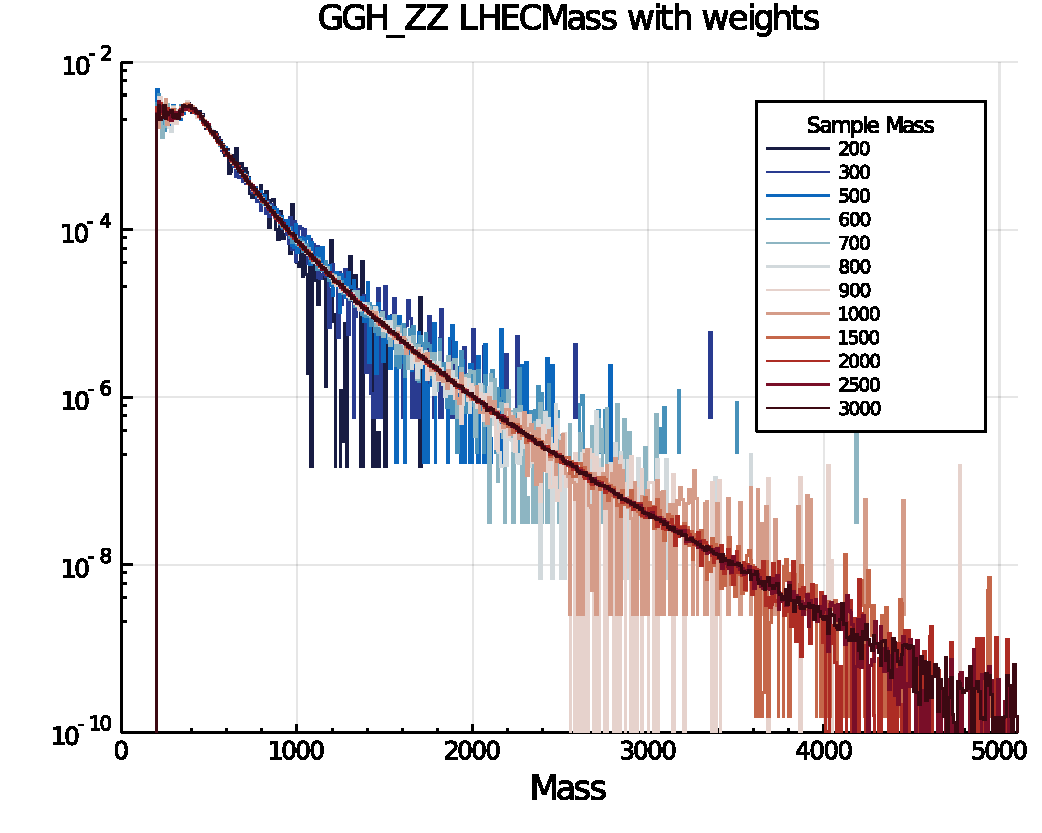
\includegraphics[width=.5\linewidth]{fig/LHE_PUME_wgts.pdf}}\\
\end{center}
\caption{Normalized distributions of LHECandMass before (left) and after (right) applying
the weights. Together they show a need to combine samples for a wide-range, high
statistics signal sample. Bin size = \SI{10}{\giga\electronvolt}.}
\label{fig:LHE_raw}
\end{figure}

The goal of the combination of samples is to use all the events, but with a correction weight
such that each sample has a higher weight in the region where they posess good statistics. Of
course while keeping the overall normalization stays unchanged. To do this, we pick a list of
`mass windows' with edges sitting on the true masses of the samples, and we define effective
number of events $\mathrm{N}_\mathrm{eff} = \frac{(\sum\mathrm{wgts})^2}{\sum(\mathrm{wgts}^2)}$
within each mass window. Here, the wgts corresponse to PU wgt, GEN wgt, K-factor, and ME weight for
the GGH sample in consideration. For a specific GGH sample $i_0$ and its events fall in a mass 
window $j$, $\mathrm{N}_\mathrm{eff}^{i_0j}$ is first obtained and a re-weighting factor can be computed:
\be
\mathrm{wgt}_\mathrm{window}^{i_0j} = 
\frac{\mathrm{N}_\mathrm{eff}^{i_0j}}{\sum_i\mathrm{N}_\mathrm{eff}^{ij}}
\ee
This factor is applied to all events from sample $i_0$ within the window $j$. Conceptually,
the effective events ensures the weight is not skewed by the difference in the overall
normalization of samples, and in each of the mass windows, samples with more concentrated
statistics in that window are given a higher weight. In Fig.~\ref{fig:window_wgt_matrix} (a), a
clear dignal pattern can be seen, physically it means that samples with higher true 
mass are given a higher weight in tail mass windows--- consistent with the expected outcome.
\begin{figure}[htb]
\begin{center}
\subfloat[]{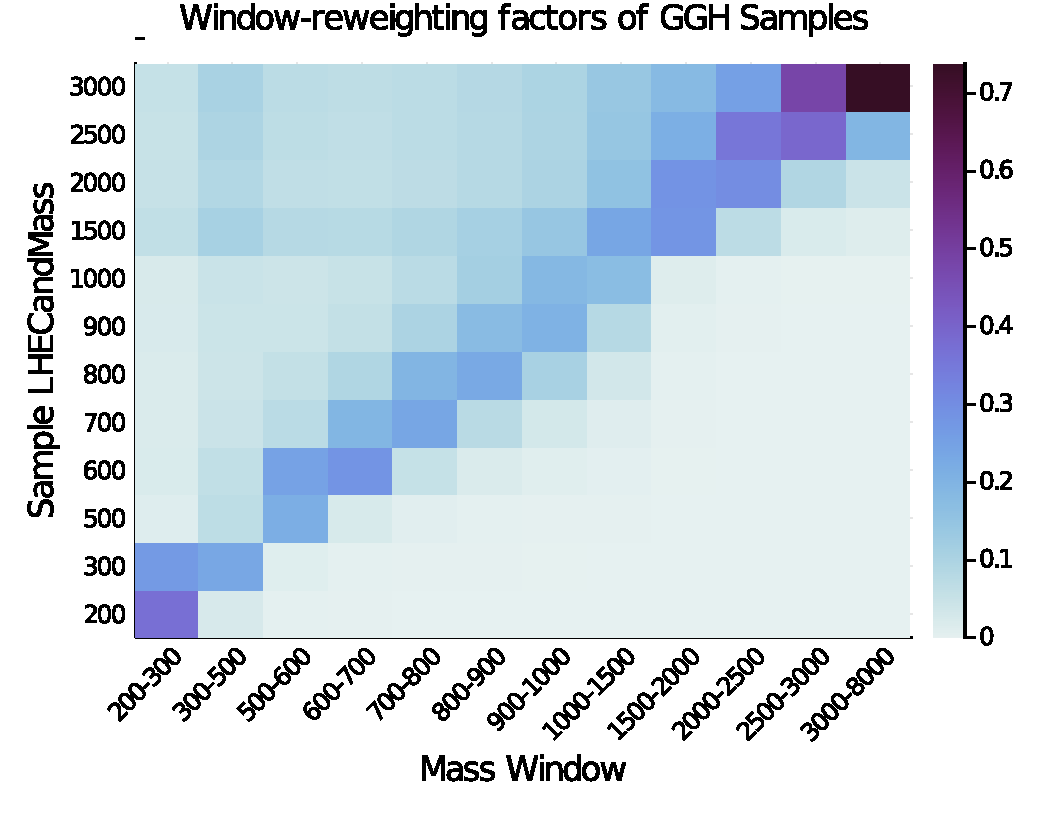
\includegraphics[width=.5\linewidth]{fig/Window_wgt_GGH.pdf}}
\subfloat[]{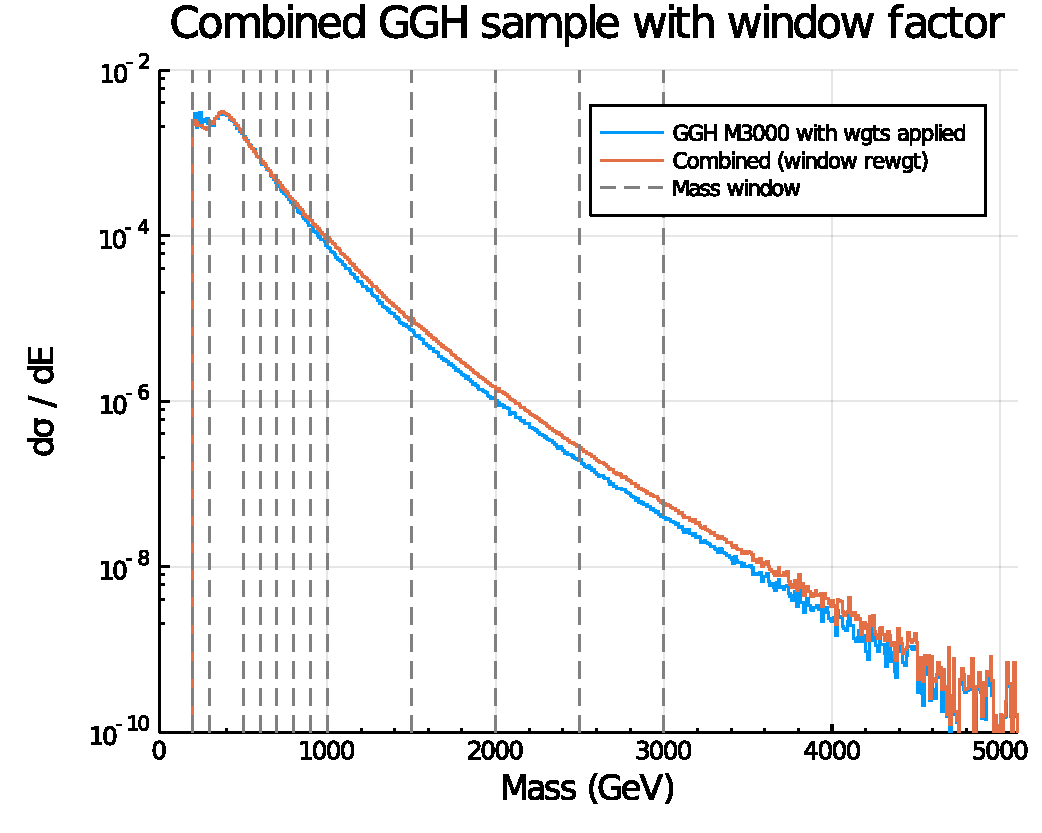
\includegraphics[width=.5\linewidth]{fig/LHC_compare_windowwgt.pdf}}
\end{center}
\caption{Heatmap of window re-weight factors of different samples and mass windows (left);
effects of applying window factors for the combined sample(right)}
\label{fig:window_wgt_matrix}
\end{figure}

However, even after the normalization, there are still inconsistency in the shape as shown
in Fig.~\ref{fig:window_wgt_matrix} (b). This is likely because the finite number of events
and non-infinitesimal mass window size used. We introduce another correction factor for
this small artifacts. Iteratively going through every sample, between the previous and the
next one, derive a sample mass factor based on:
\be
\mathrm{wgt}_\mathrm{mass}^{i, i+1} = \frac{\sum{\mathrm{wgt}_\mathrm{i}}}{\sum{\mathrm{wgt}_\mathrm{i+1}}}
\text{, for events that has Mass between sample mass of $i$ and $i+1$}
\ee

\begin{figure}[htb]
\begin{center}
\subfloat[]{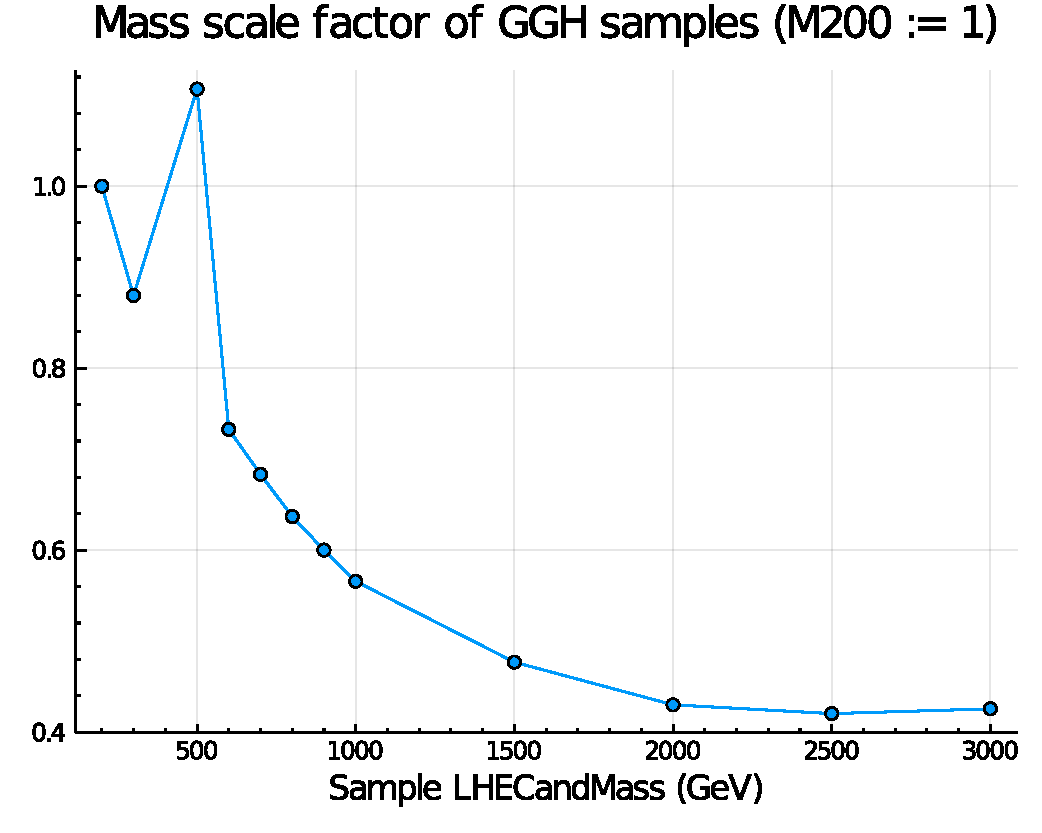
\includegraphics[width=.5\linewidth]{fig/Mass_wgt_GGH.pdf}}
\subfloat[]{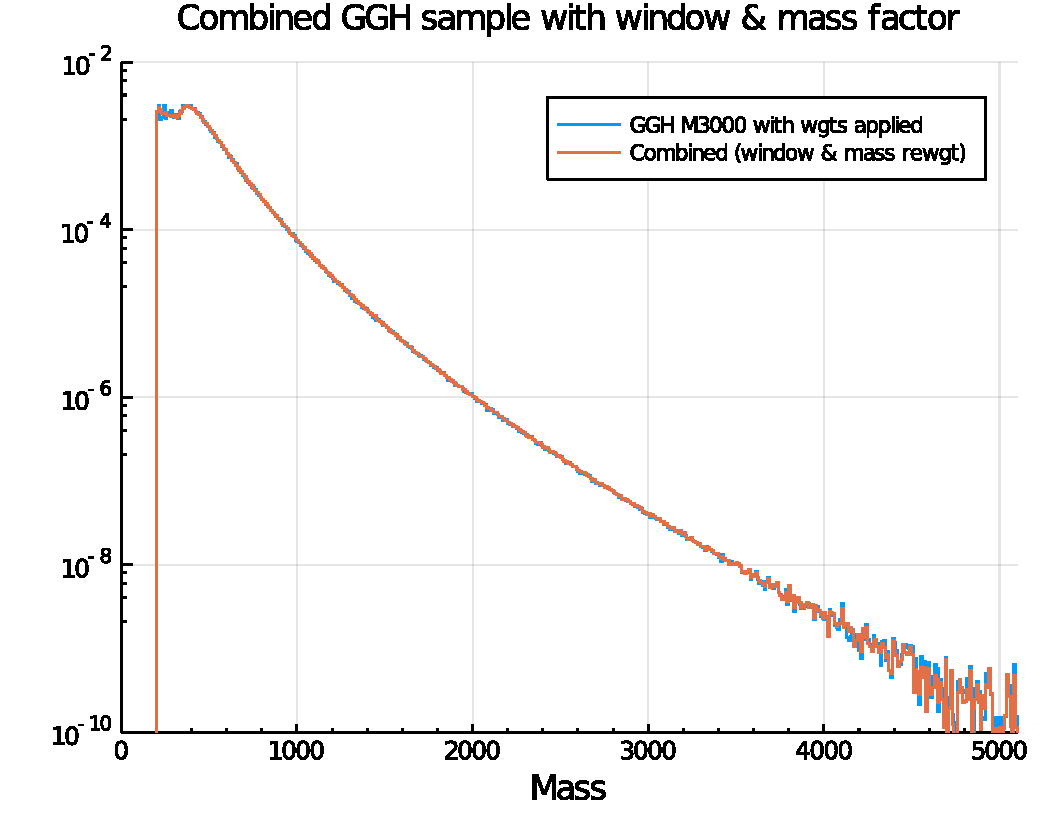
\includegraphics[width=.5\linewidth]{fig/LHC_compare_bothwgt.pdf}}
\end{center}
\caption{Iterative sample mass factors obtained (left) and the final combined sample (right)}
\label{fig:LHE_rewgt}
\end{figure}

This factor corrects the high variations of overall normalizations between samples, the factors and result
are shown in Fig.~\ref{fig:LHE_rewgt}. As expected, high mass samples need a down correction (not by a lot)
to eliminate the deviated trend before.

Finally, although we used the matrix element weights for one of the signal hypothesis, these two
correction factors apply too all hypothesis and a plot of them without normalization are shown
in Fig.~\ref{fig:bsi_sig_bkg_compare}. As expected, background dominates by almost an order of
magnitude which is why the constrain is hard to obtain.

\begin{figure}[htb]
\begin{center}
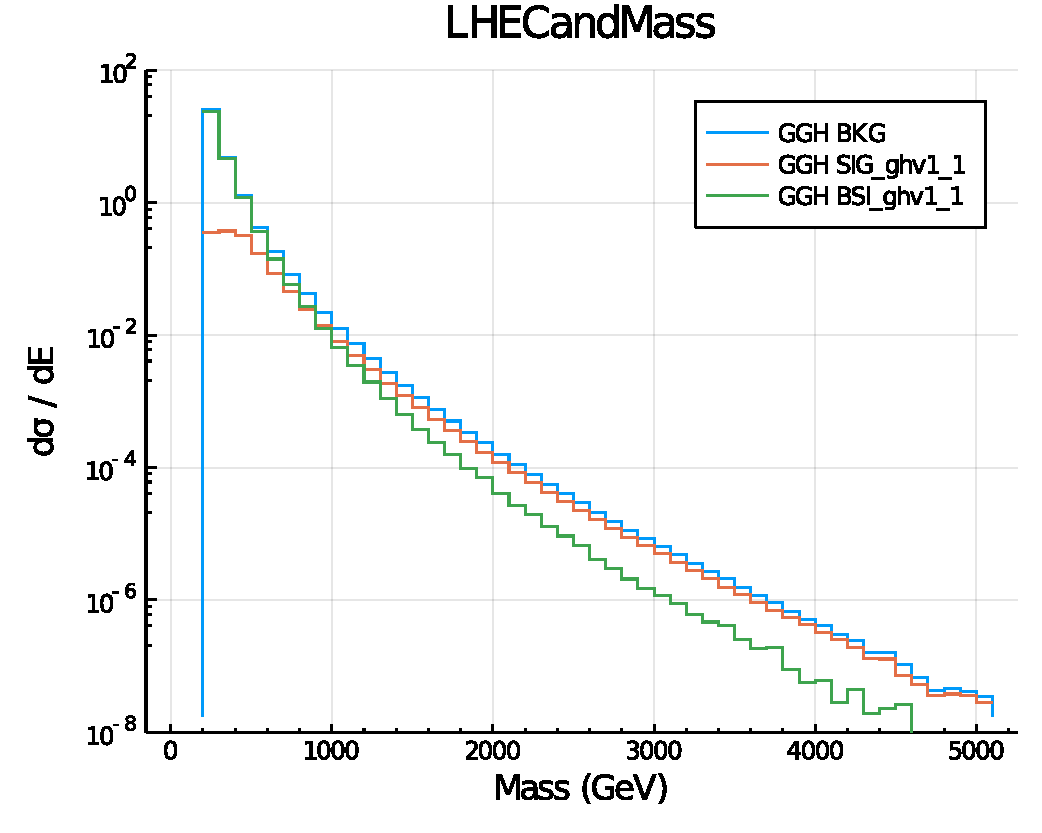
\includegraphics[width=.8\linewidth]{fig/LHE_integral_difference.pdf}
\end{center}
\caption{Distributions of background, signal, and background signal interaction}
\label{fig:bsi_sig_bkg_compare}
\end{figure}


\section{Strategy in variable selection and binning}
\begin{figure}[htb]
\begin{center}
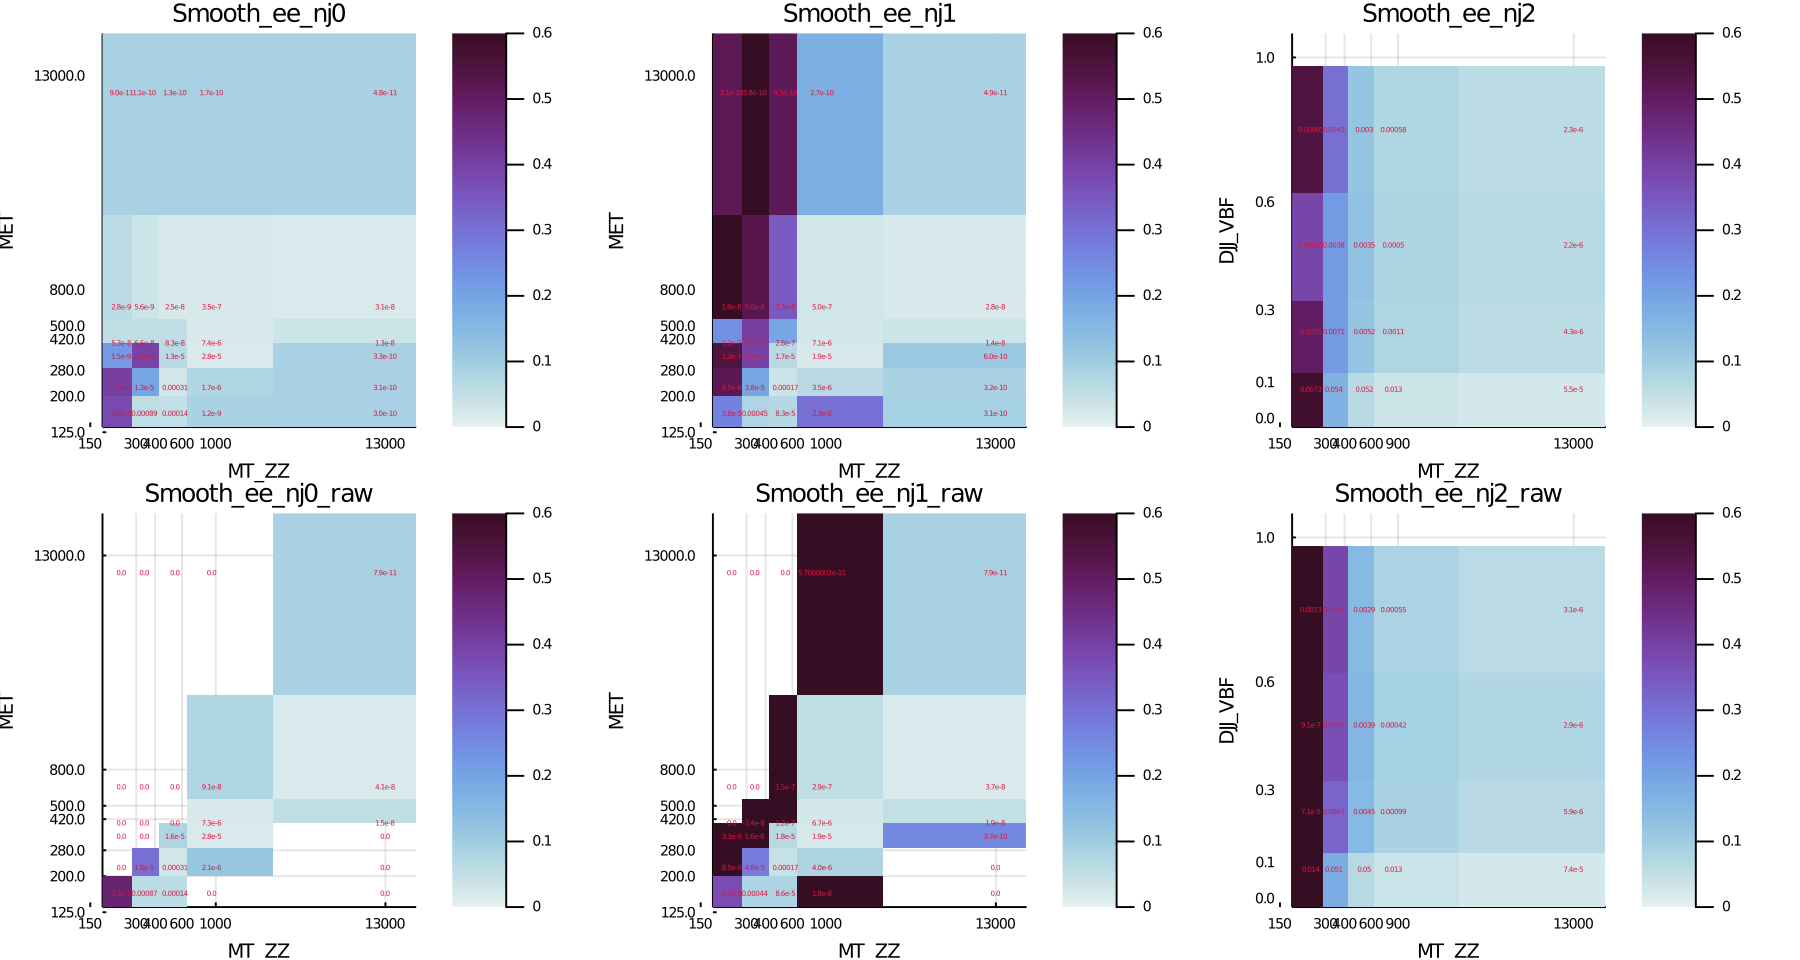
\includegraphics[width=.90\linewidth]{fig/binning_placeholder.png}
\end{center}
\label{fig:sig_rewgt}
\end{figure}
\todo[inline]{make plots publication quality and give quantitative justification for choice}
